\chapter{Design Pattern}
\section{DAO Pattern}
\medskip
Per quanto riguarda la logica di accesso alla sorgente di dati, si è deciso di utilizzare il pattern DAO.

L'idea del pattern DAO (Data Access Object) è di disaccoppiare la logica di business dalla logica di accesso ai dati. Questo si ottiene spostando la logica di accesso ai dati dai componenti di business ad una classe DAO. Questo approccio garantisce che un eventuale cambiamento del dispositivo di persistenza non comporti modifiche sui componenti di business.

Esiste una classe DAO per ogni classe che rappresenta entità del dominio di applicazione. Questa classe conterrà i metodi di integrazione e manipolazione della corrispondente classe di dominio. In particolare conterrà le funzionalità di base CRUD.
\begin{itemize}
\item Create
\item Read
\item Update
\item Delete
\end{itemize}
\subsection*{Struttura}
Il DAO viene invocato dal Business Object e si occupa di effettuare l'accesso ai dati restituendoli all'applicazione.\\

Le informazioni che il DAO restituisce al Business Object sono oggetti generici, indipendenti dal dispositivo di persistenza, e le eventuali eccezioni specifiche della risorsa dati sono mascherate in eccezioni generiche di tipo applicativo.

\begin{figure}[tb]
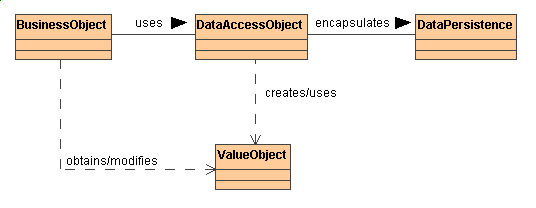
\includegraphics[width=\textwidth]{img/patternDao.jpg} 
\caption{Struttura del Pattern DAO}
\end{figure}

